\subsection{Выводы}
\label{sec:optimization:notes}

Сделаем выводы по проделанной работе. В качестве результатов можно привести три характерных графика. Они отражают суть оптимизации для трех типов запросов, на которые можно поделить все общение с базой:

\begin{itemize}
  \item Запросы, возвращающие большие объемы данных, в том числе включающие в себя много агрегированных значений. Примером такого вида запросов является \lstinline{resultByProduct} (график \ref{fig:optimization:notes:result_by_product}), который собирает большое количество характеристик и отображает в виде таблицы (таблица с около 20ю колонками), включающие средние/общие продажы, количество \emph{lost sales}, параметры привоза товара и тп. До оптимизации среднее время ответа варьировалось между $4-4.5 c$, после - $1-2 с$.
  \item Мелкие запросы. Не представляют собой сложные вычисления. Пример - отфильтрованный по одному товару с небольшим количеством возвращаемой информации \lstinline{resultByProduct} (график \ref{fig:optimization:notes:result_by_product_filtered}). Как до, так и после оптимизации среднее время ответа невелико - $0.4-0.5 с$.
  \item Сложное обновление. Таких запросов всего в приложении несколько штук, одним из них является изменение даты начала продаж у магазина (\lstinline{store_start_selling_date}) (график \ref{fig:optimization:notes:store_start_selling_date_update}). Изменение этого значения влечет за собой пересчет всего планируемого цикла продаж. До оптимизации запрос на обновление этого параметра для выбранного магазина отрабатывал более чем за $10$ секунд. После оптимизации - в среднем $4-5$ секунды.
\end{itemize}

\begin{figure}
	\centering
	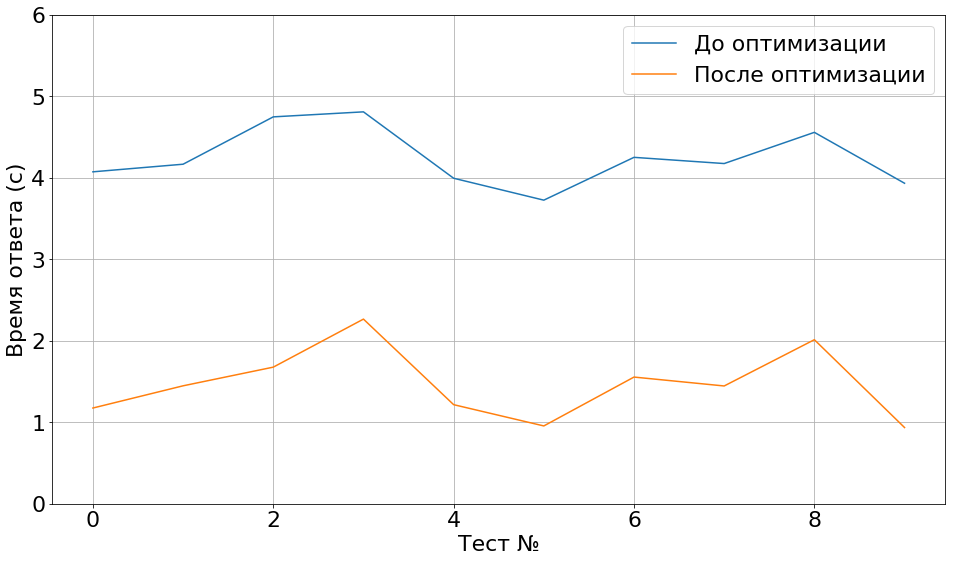
\includegraphics[scale=0.47]{resultByProduct.png}
	\caption{Сравнительный график времени выполнения запроса \lstinline{resultByProduct} до оптимизации и после}
	\label{fig:optimization:notes:result_by_product}
\end{figure}

\begin{figure}
	\centering
	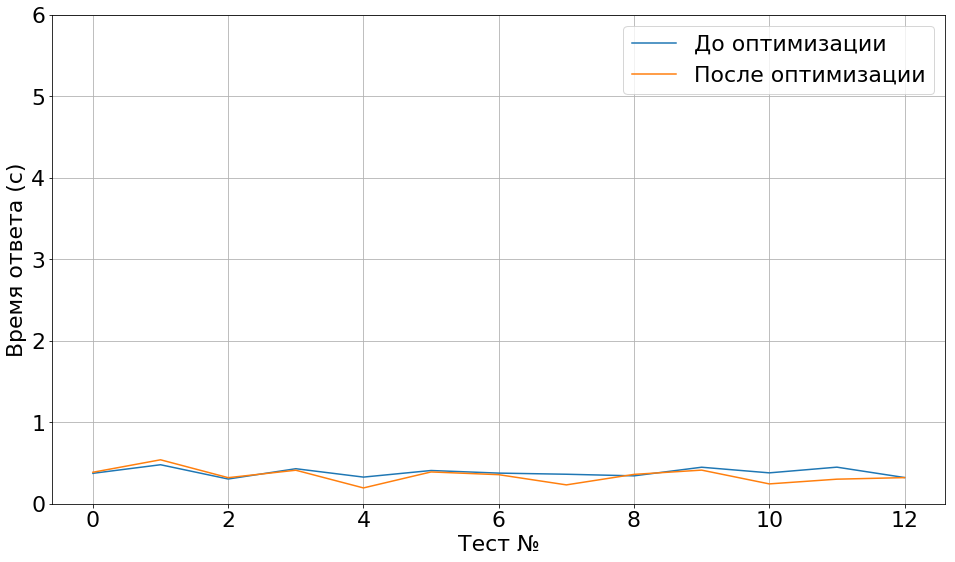
\includegraphics[scale=0.47]{resultByProduct_filtered.png}
	\caption{Сравнительный график времени выполнения запроса упрощенного  \lstinline{resultByProduct} для одного товара до оптимизации и после}
	\label{fig:optimization:notes:result_by_product_filtered}
\end{figure}

\begin{figure}
	\centering
	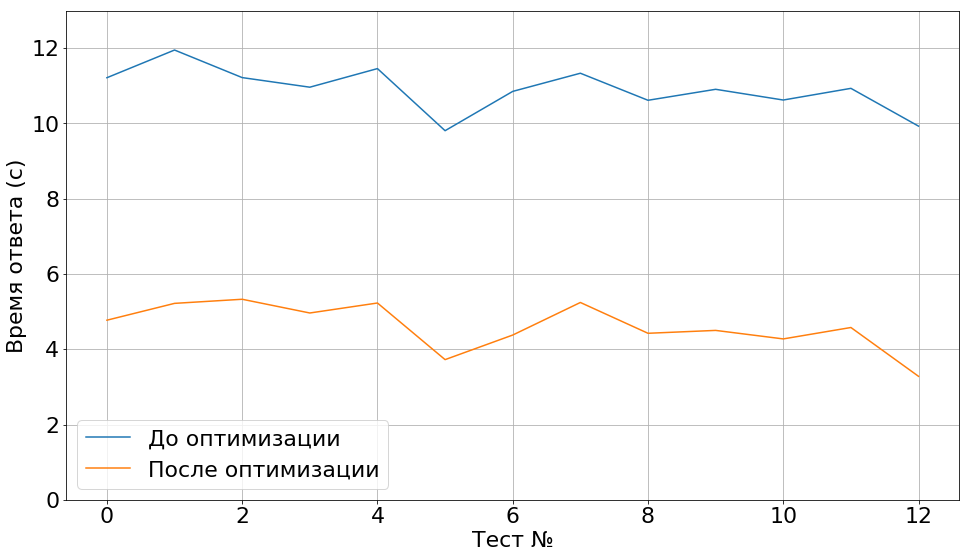
\includegraphics[scale=0.47]{store_start_selling_date_update.png}
	\caption{Сравнительный график времени выполнения обновления даты начала продаж для магазина до оптимизации и после}
	\label{fig:optimization:notes:store_start_selling_date_update}
\end{figure}

Если же попытаться кратко упомянуть все найденные возможности для оптимизации платформы \LB и вместить в один список, то получится нечто следующее:

\begin{itemize}
  \item компилятор переписывает сложные формулы с функциональными предикатами и операторами сравнения в атомарные инструкции;
  \item выбранный порядок ключей при операциях \join часто является причиной длительных запросов (\emph{long-running rules}). Такие случаи легко выявить при изучении ключей в исходном правиле;
  \item некоторые правила выходят за рамки линейной асимптотики, что плохо сказывается на производительности из-за большого количества исходных данных;
  \item следует избегать правил, которые делают \join по временным объектам, используя неравенства. Вместо этого лучше использовать конструкцию \lstinline{int:range};
  \item стоит хорошо называть промежуточные предикаты, введенные для оптимизации (при переформулировке правил), а также добавлять соответствующие комментарии к ним, чтобы с течением времени эти изменения не были удалены и по-прежнему были понятны;
  \item при использовании \lstinline{force_key_ordering} pragma стоит ставить меньше ключей, чтобы меньше ограничивать оптимизатор;
  \item полезно придерживаться одного шаблона при pragma, например часто используется следующий формат: $"pragma" + $ \lstinline{string} $ +$\linebreak $ "force\_key\_ordering"$;
  \item запись в логах, содержащая \lstinline{long-running "ExUnRule"}, указывает на блок и номер строки с самой long-running rule;
  \item чтобы вывести самые долгие правила, необходимы выполнить \lstinline{grep took lb-server.log |}\lstinline| awk '{print $(NF-1) " " $0;}'|\lstinline{ | sort -r -n|}
  \item настройка окружения \lstinline{LB_SUPPRESS_TASK_PARALLELISM=1} помогает логу быть в едином потоке, в противном случае записи будут находиться в хаотичном порядке;
  \item стоит помнить об автоматическом создании и удалении индексов
\end{itemize}
